   \begin{figure}[h]
        \centering
		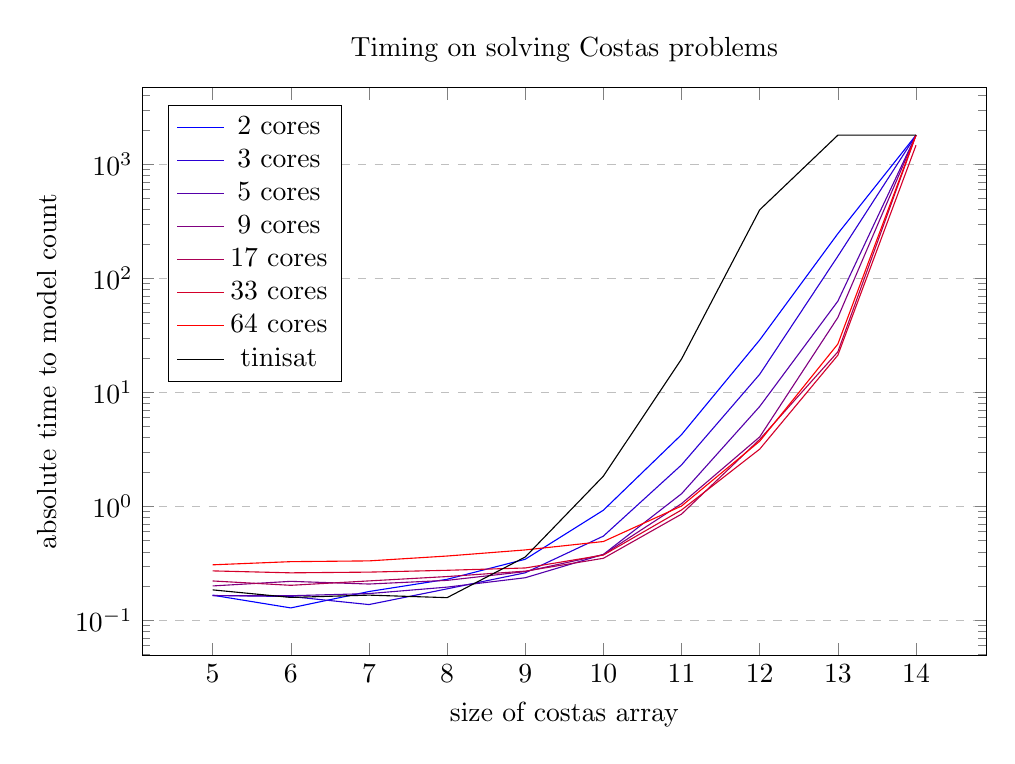
\begin{tikzpicture}
		\begin{axis}[
			title={Timing on solving Costas problems},
			xlabel={size of costas array},
			ylabel={absolute time to model count},
			%xmin=0, xmax=0.25,
			%ymin=10.00, ymax=100000.00,
			ymode=log,
			%xmode=log,
			%xtick={0,0.05,0.1,0.15,0.2,0.25},
			%ytick={0,20,40,60,80,100},
			%yticklabel=$\pgfmathprintnumber{\tick}\%$,
			legend pos=north west,
			ymajorgrids=true,
			grid style=dashed,
			xticklabel style={/pgf/number format/fixed},
			width = 350,
			height = 250
		]






\addplot[color=red!0.0!blue,line width=0.4pt] coordinates {
(5,0.16651105880737305)(6,0.128767728805542)(7,0.17928266525268555)(8,0.229478120803833)(9,0.3440828323364258)(10,0.9262895584106445)(11,4.26284122467041)(12,28.817259788513184)(13,246.72397589683533)(14,1801.013244152069)
}node[pos=0.8](endofplotsquare){} ;
\addlegendentry{2 cores}
\addplot[color=red!16.666666666666668!blue,line width=0.4pt] coordinates {
(5,0.16553544998168945)(6,0.16209650039672852)(7,0.1377730369567871)(8,0.18923521041870117)(9,0.2616755962371826)(10,0.5489482879638672)(11,2.313494920730591)(12,14.413764238357544)(13,156.3844666481018)(14,1801.0142397880554)
}node[pos=0.8](endofplotsquare){} ;
\addlegendentry{3 cores}
\addplot[color=red!33.333333333333336!blue,line width=0.4pt] coordinates {
(5,0.164872407913208)(6,0.16470789909362793)(7,0.17198729515075684)(8,0.19599699974060059)(9,0.23682069778442383)(10,0.3795149326324463)(11,1.291374921798706)(12,7.523766040802002)(13,63.10072612762451)(14,1801.0149838924408)
}node[pos=0.8](endofplotsquare){} ;
\addlegendentry{5 cores}
\addplot[color=red!50.0!blue,line width=0.4pt] coordinates {
(5,0.20067811012268066)(6,0.22022223472595215)(7,0.20856070518493652)(8,0.22462010383605957)(9,0.2682313919067383)(10,0.37816452980041504)(11,1.0574686527252197)(12,4.069439888000488)(13,45.39408540725708)(14,1801.0188295841217)
}node[pos=0.8](endofplotsquare){} ;
\addlegendentry{9 cores}
\addplot[color=red!66.66666666666667!blue,line width=0.4pt] coordinates {
(5,0.22196483612060547)(6,0.2032465934753418)(7,0.22217583656311035)(8,0.24254584312438965)(9,0.2705719470977783)(10,0.35074734687805176)(11,0.8557615280151367)(12,3.8713788986206055)(13,22.67898917198181)(14,1801.0271427631378)
}node[pos=0.8](endofplotsquare){} ;
\addlegendentry{17 cores}
\addplot[color=red!83.33333333333333!blue,line width=0.4pt] coordinates {
(5,0.2719554901123047)(6,0.2614936828613281)(7,0.2652904987335205)(8,0.27526402473449707)(9,0.28845834732055664)(10,0.37433934211730957)(11,0.9312081336975098)(12,3.1793856620788574)(13,21.185994863510132)(14,1469.3303191661835)
}node[pos=0.8](endofplotsquare){} ;
\addlegendentry{33 cores}
\addplot[color=red!100.0!blue,line width=0.4pt] coordinates {
(5,0.3074929714202881)(6,0.32775092124938965)(7,0.33288002014160156)(8,0.36718130111694336)(9,0.415346622467041)(10,0.4921422004699707)(11,1.0077219009399414)(12,3.730285882949829)(13,26.540127277374268)(14,1802.017567873001)
}node[pos=0.8](endofplotsquare){} ;
\addlegendentry{64 cores}
\addplot[color=black,line width=0.4pt] coordinates {
(5,0.18535566329956055)(6,0.15912103652954102)(7,0.16672492027282715)(8,0.15842223167419434)(9,0.36010169982910156)(10,1.843733787536621)(11,19.61815071105957)(12,398.9100785255432)(13,1801.0124578475952)(14,1801.01256108284)
}node[pos=0.8](endofplotsquare){} ;
\addlegendentry{tinisat}

		\end{axis}
		\end{tikzpicture}
		%\vspace{-18pt}
		\caption[Runtime to solve Costas arrays]{Runtime to solve Costas arrays, by core count and costas array size w/ 1800s timeout}
		\label{fig:performance_graph3}
    \end{figure}
